\documentclass{article}\usepackage[]{graphicx}\usepackage[]{xcolor}
% maxwidth is the original width if it is less than linewidth
% otherwise use linewidth (to make sure the graphics do not exceed the margin)
\makeatletter
\def\maxwidth{ %
  \ifdim\Gin@nat@width>\linewidth
    \linewidth
  \else
    \Gin@nat@width
  \fi
}
\makeatother

\definecolor{fgcolor}{rgb}{0.345, 0.345, 0.345}
\newcommand{\hlnum}[1]{\textcolor[rgb]{0.686,0.059,0.569}{#1}}%
\newcommand{\hlstr}[1]{\textcolor[rgb]{0.192,0.494,0.8}{#1}}%
\newcommand{\hlcom}[1]{\textcolor[rgb]{0.678,0.584,0.686}{\textit{#1}}}%
\newcommand{\hlopt}[1]{\textcolor[rgb]{0,0,0}{#1}}%
\newcommand{\hlstd}[1]{\textcolor[rgb]{0.345,0.345,0.345}{#1}}%
\newcommand{\hlkwa}[1]{\textcolor[rgb]{0.161,0.373,0.58}{\textbf{#1}}}%
\newcommand{\hlkwb}[1]{\textcolor[rgb]{0.69,0.353,0.396}{#1}}%
\newcommand{\hlkwc}[1]{\textcolor[rgb]{0.333,0.667,0.333}{#1}}%
\newcommand{\hlkwd}[1]{\textcolor[rgb]{0.737,0.353,0.396}{\textbf{#1}}}%
\let\hlipl\hlkwb

\usepackage{framed}
\makeatletter
\newenvironment{kframe}{%
 \def\at@end@of@kframe{}%
 \ifinner\ifhmode%
  \def\at@end@of@kframe{\end{minipage}}%
  \begin{minipage}{\columnwidth}%
 \fi\fi%
 \def\FrameCommand##1{\hskip\@totalleftmargin \hskip-\fboxsep
 \colorbox{shadecolor}{##1}\hskip-\fboxsep
     % There is no \\@totalrightmargin, so:
     \hskip-\linewidth \hskip-\@totalleftmargin \hskip\columnwidth}%
 \MakeFramed {\advance\hsize-\width
   \@totalleftmargin\z@ \linewidth\hsize
   \@setminipage}}%
 {\par\unskip\endMakeFramed%
 \at@end@of@kframe}
\makeatother

\definecolor{shadecolor}{rgb}{.97, .97, .97}
\definecolor{messagecolor}{rgb}{0, 0, 0}
\definecolor{warningcolor}{rgb}{1, 0, 1}
\definecolor{errorcolor}{rgb}{1, 0, 0}
\newenvironment{knitrout}{}{} % an empty environment to be redefined in TeX

\usepackage{alltt}
\usepackage{fullpage}
\usepackage{textcomp}
\usepackage{enumitem}
\usepackage{graphicx}


\title{STstuff package vignette}
\author{David Venet}
\date{\today}
\IfFileExists{upquote.sty}{\usepackage{upquote}}{}
\begin{document}
\maketitle
   
   
\section{Introduction}
%%%%%%%%%%%%%%%%%%%%%%%%%%%%%%%%%

\section{Simulation}
%%%%%%%%%%%%%%%%%%%%%%%%
We simulate data, where each spot is a mixture of 3 basic vectors.
Those vectors are chosen to be correlated, as gene expression is.
The parameters of the mixture are taken from a Dirichlet distribution, so that they are often close to 1 but not always.
Then we take the mixture from each spot as the mean of a negative binomial and draw random values from there.
  
\begin{knitrout}
\definecolor{shadecolor}{rgb}{0.969, 0.969, 0.969}\color{fgcolor}\begin{kframe}
\begin{alltt}
\hlkwd{library}\hlstd{(STstuff);}

\hlkwd{library}\hlstd{(dirmult);} \hlcom{# for the Dirichlet (in the simulation)}

\hlstd{Nprot} \hlkwb{=} \hlnum{3}\hlstd{; Nspot} \hlkwb{=} \hlnum{100}\hlopt{*}\hlstd{Nprot;}
\hlstd{Ngene} \hlkwb{=} \hlnum{500}\hlstd{;}
\hlstd{gb} \hlkwb{=} \hlkwd{rexp}\hlstd{(Ngene)}\hlopt{^}\hlnum{2}\hlopt{+}\hlnum{1}\hlstd{;} \hlcom{# Gene specific values}
\hlstd{prot} \hlkwb{=} \hlkwd{matrix}\hlstd{(}\hlkwd{rexp}\hlstd{(Ngene}\hlopt{*}\hlstd{Nprot),} \hlkwc{ncol}\hlstd{=Nprot)} \hlopt{*} \hlstd{gb;} \hlcom{# prototypes}
\hlstd{protl} \hlkwb{=} \hlkwd{log}\hlstd{(}\hlnum{1}\hlopt{+}\hlnum{1e4}\hlopt{*}\hlkwd{t}\hlstd{(prot)}\hlopt{/}\hlkwd{colSums}\hlstd{(prot))}
\hlstd{mix} \hlkwb{=} \hlkwd{rdirichlet}\hlstd{(Nspot,} \hlkwc{alpha}\hlstd{=}\hlkwd{c}\hlstd{(}\hlnum{1}\hlstd{,}\hlnum{1}\hlstd{,}\hlnum{1}\hlstd{)}\hlopt{*}\hlnum{.1}\hlstd{)} \hlcom{# Mixture from all 3 classes for each spot}
\hlstd{base} \hlkwb{=} \hlstd{mix} \hlopt \hlkwd{t}\hlstd{(prot)}
\hlstd{X} \hlkwb{=} \hlkwd{matrix}\hlstd{(}\hlkwd{rnbinom}\hlstd{(base,} \hlkwc{mu}\hlstd{=base,} \hlkwc{size}\hlstd{=}\hlnum{1}\hlstd{),} \hlkwc{ncol}\hlstd{=}\hlkwd{ncol}\hlstd{(base));}
\end{alltt}
\end{kframe}
\end{knitrout}

The distribution of the mix is often close to 0 or 1, as wanted.
\begin{knitrout}
\definecolor{shadecolor}{rgb}{0.969, 0.969, 0.969}\color{fgcolor}\begin{kframe}
\begin{alltt}
\hlkwd{hist}\hlstd{(mix[,}\hlnum{1}\hlstd{],} \hlkwc{breaks}\hlstd{=}\hlnum{30}\hlstd{)}
\end{alltt}
\end{kframe}
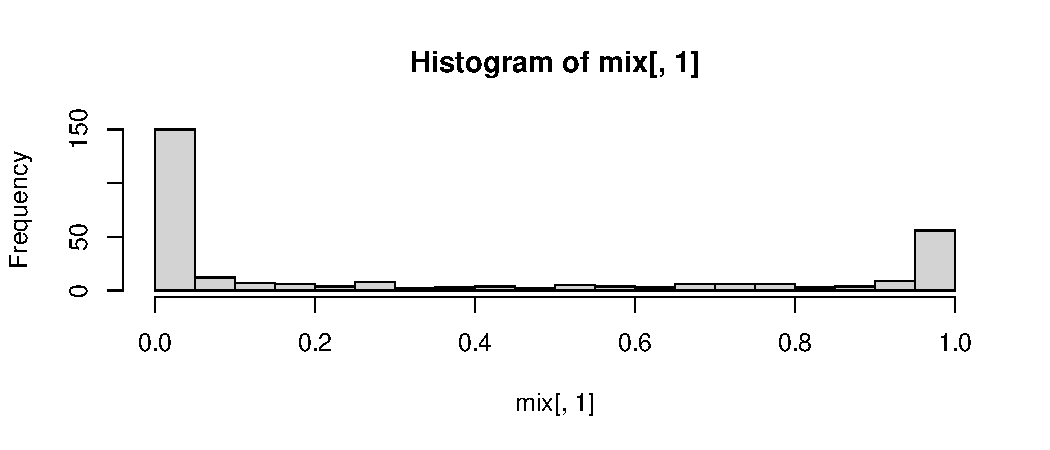
\includegraphics[width=\maxwidth]{figure/plotHistMix-1} 
\end{knitrout}

From here, we first do a kmeans to get the clusters.
We start from the real prototype to ensure that we get the right ordering.

\begin{knitrout}
\definecolor{shadecolor}{rgb}{0.969, 0.969, 0.969}\color{fgcolor}\begin{kframe}
\begin{alltt}
\hlstd{y} \hlkwb{=} \hlkwd{log}\hlstd{(}\hlnum{1}\hlopt{+}\hlnum{1e4}\hlopt{*}\hlstd{X}\hlopt{/}\hlkwd{rowSums}\hlstd{(X))}
\hlstd{km} \hlkwb{=} \hlkwd{kmeans}\hlstd{(y, protl);}
\end{alltt}
\end{kframe}
\end{knitrout}

We can see that the cluster centers, although correlated to the correct prototypes, are also correlated to each other.

\begin{knitrout}
\definecolor{shadecolor}{rgb}{0.969, 0.969, 0.969}\color{fgcolor}\begin{kframe}
\begin{alltt}
\hlstd{pr} \hlkwb{=} \hlkwd{t}\hlstd{(km}\hlopt{$}\hlstd{centers)}
\hlstd{prO} \hlkwb{=} \hlstd{(}\hlkwd{exp}\hlstd{(pr)}\hlopt{-}\hlnum{1}\hlstd{)}\hlopt{*}\hlkwd{colSums}\hlstd{(prot)}\hlopt{/}\hlnum{1e4}\hlstd{;}

\hlkwd{par}\hlstd{(}\hlkwc{mfrow}\hlstd{=}\hlkwd{c}\hlstd{(}\hlnum{3}\hlstd{,}\hlnum{3}\hlstd{),} \hlkwc{mar}\hlstd{=}\hlkwd{c}\hlstd{(}\hlnum{3}\hlstd{,}\hlnum{3}\hlstd{,}\hlnum{.5}\hlstd{,}\hlnum{.5}\hlstd{),} \hlkwc{mgp}\hlstd{=}\hlkwd{c}\hlstd{(}\hlnum{1.5}\hlstd{,}\hlnum{.5}\hlstd{,}\hlnum{0}\hlstd{))}
\hlkwa{for} \hlstd{(i} \hlkwa{in} \hlnum{1}\hlopt{:}\hlnum{3}\hlstd{)}
\hlstd{\{} \hlkwa{for} \hlstd{(j} \hlkwa{in} \hlnum{1}\hlopt{:}\hlnum{3}\hlstd{)}
  \hlstd{\{} \hlkwd{plot}\hlstd{(prot[,i], prO[,j],} \hlkwc{log}\hlstd{=}\hlstr{'xy'}\hlstd{,} \hlkwc{xlab}\hlstd{=}\hlkwd{paste}\hlstd{(}\hlstr{"Recovered proto"}\hlstd{, i),}
      \hlkwc{ylab}\hlstd{=}\hlkwd{paste}\hlstd{(}\hlstr{"Real proto"}\hlstd{, j));} \hlcom{#abline(0,1)}
    \hlkwd{mtext}\hlstd{(}\hlkwd{paste0}\hlstd{(}\hlstr{"Cor:"}\hlstd{,} \hlkwd{round}\hlstd{(}\hlkwd{cor}\hlstd{(prot[,i], pr[,j],} \hlkwc{method}\hlstd{=}\hlstr{'s'}\hlstd{)}\hlopt{*}\hlnum{100}\hlstd{),} \hlstr{"%"}\hlstd{),} \hlkwc{side}\hlstd{=}\hlnum{3}\hlstd{,} \hlkwc{line}\hlstd{=}\hlopt{-}\hlnum{2}\hlstd{)}
  \hlstd{\}}
\hlstd{\}}
\end{alltt}


{\ttfamily\noindent\color{warningcolor}{\#\# Warning in xy.coords(x, y, xlabel, ylabel, log): 1 y value <= 0 omitted from logarithmic plot}}

{\ttfamily\noindent\color{warningcolor}{\#\# Warning in xy.coords(x, y, xlabel, ylabel, log): 1 y value <= 0 omitted from logarithmic plot}}

{\ttfamily\noindent\color{warningcolor}{\#\# Warning in xy.coords(x, y, xlabel, ylabel, log): 1 y value <= 0 omitted from logarithmic plot}}\end{kframe}
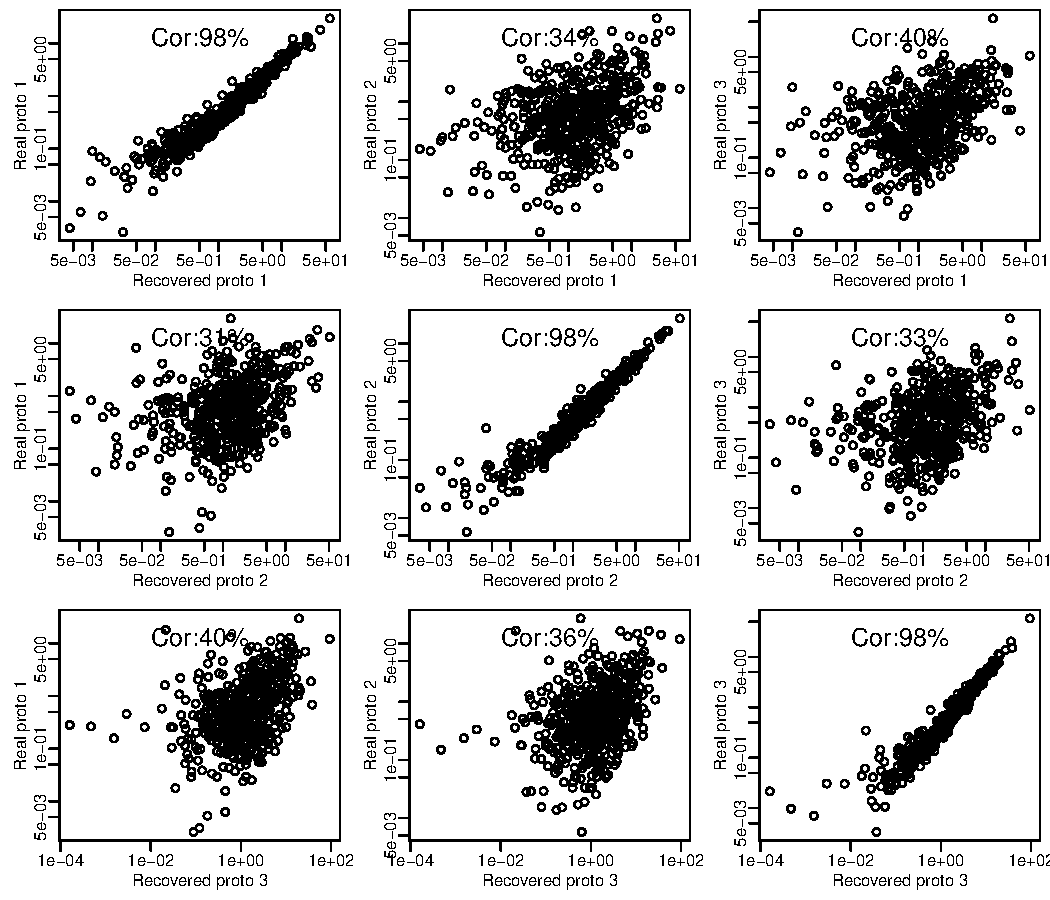
\includegraphics[width=\maxwidth]{figure/plotCorKM-1} 
\end{knitrout}

We can deconvolute the cluster.

\begin{knitrout}
\definecolor{shadecolor}{rgb}{0.969, 0.969, 0.969}\color{fgcolor}\begin{kframe}
\begin{alltt}
\hlstd{deconv} \hlkwb{=} \hlkwd{NNMFfromKM}\hlstd{(X, km}\hlopt{$}\hlstd{cluster,} \hlkwc{Niter}\hlstd{=}\hlnum{10}\hlstd{,} \hlkwc{mccores}\hlstd{=}\hlnum{7}\hlstd{)}
\end{alltt}


{\ttfamily\noindent\itshape\color{messagecolor}{\#\# \ \ \ \ \ Iter:1}}

{\ttfamily\noindent\itshape\color{messagecolor}{\#\# \ \ \ \ \ Iter:2}}

{\ttfamily\noindent\itshape\color{messagecolor}{\#\# \ \ \ \ \ Iter:3}}

{\ttfamily\noindent\itshape\color{messagecolor}{\#\# \ \ \ \ \ Iter:4}}

{\ttfamily\noindent\itshape\color{messagecolor}{\#\# \ \ \ \ \ Iter:5}}

{\ttfamily\noindent\itshape\color{messagecolor}{\#\# \ \ \ \ \ Iter:6}}

{\ttfamily\noindent\itshape\color{messagecolor}{\#\# \ \ \ \ \ Iter:7}}

{\ttfamily\noindent\itshape\color{messagecolor}{\#\# \ \ \ \ \ Iter:8}}

{\ttfamily\noindent\itshape\color{messagecolor}{\#\# \ \ \ \ \ Iter:9}}

{\ttfamily\noindent\itshape\color{messagecolor}{\#\# \ \ \ \ \ Iter:10}}\begin{alltt}
\hlstd{pr2} \hlkwb{=} \hlstd{deconv}\hlopt{$}\hlstd{proto;} \hlcom{# pr2 are the new prototypes}
\end{alltt}
\end{kframe}
\end{knitrout}

The new prototypes are still well correlated with the real prototypes, but they are also less correlated to each other.
Note that some correlation is still expected because the original prototypes are also correlated.

\begin{knitrout}
\definecolor{shadecolor}{rgb}{0.969, 0.969, 0.969}\color{fgcolor}\begin{kframe}
\begin{alltt}
\hlkwd{par}\hlstd{(}\hlkwc{mfrow}\hlstd{=}\hlkwd{c}\hlstd{(}\hlnum{3}\hlstd{,}\hlnum{3}\hlstd{),} \hlkwc{mar}\hlstd{=}\hlkwd{c}\hlstd{(}\hlnum{3}\hlstd{,}\hlnum{3}\hlstd{,}\hlnum{.5}\hlstd{,}\hlnum{.5}\hlstd{),} \hlkwc{mgp}\hlstd{=}\hlkwd{c}\hlstd{(}\hlnum{1.5}\hlstd{,}\hlnum{.5}\hlstd{,}\hlnum{0}\hlstd{))}
\hlkwa{for} \hlstd{(i} \hlkwa{in} \hlnum{1}\hlopt{:}\hlnum{3}\hlstd{)}
\hlstd{\{} \hlkwa{for} \hlstd{(j} \hlkwa{in} \hlnum{1}\hlopt{:}\hlnum{3}\hlstd{)}
  \hlstd{\{} \hlkwd{plot}\hlstd{(prot[,i], pr2[,j],} \hlkwc{xlab}\hlstd{=}\hlkwd{paste}\hlstd{(}\hlstr{"Recovered proto"}\hlstd{, i),}
      \hlkwc{ylab}\hlstd{=}\hlkwd{paste}\hlstd{(}\hlstr{"Real proto"}\hlstd{, j));} \hlkwd{abline}\hlstd{(}\hlnum{0}\hlstd{,}\hlnum{1}\hlstd{)}
    \hlkwd{mtext}\hlstd{(}\hlkwd{paste0}\hlstd{(}\hlstr{"Cor:"}\hlstd{,} \hlkwd{round}\hlstd{(}\hlkwd{cor}\hlstd{(prot[,i], pr2[,j],} \hlkwc{method}\hlstd{=}\hlstr{'s'}\hlstd{)}\hlopt{*}\hlnum{100}\hlstd{),} \hlstr{"%"}\hlstd{),} \hlkwc{side}\hlstd{=}\hlnum{3}\hlstd{,} \hlkwc{line}\hlstd{=}\hlopt{-}\hlnum{2}\hlstd{)}
  \hlstd{\}}
\hlstd{\}}
\end{alltt}
\end{kframe}
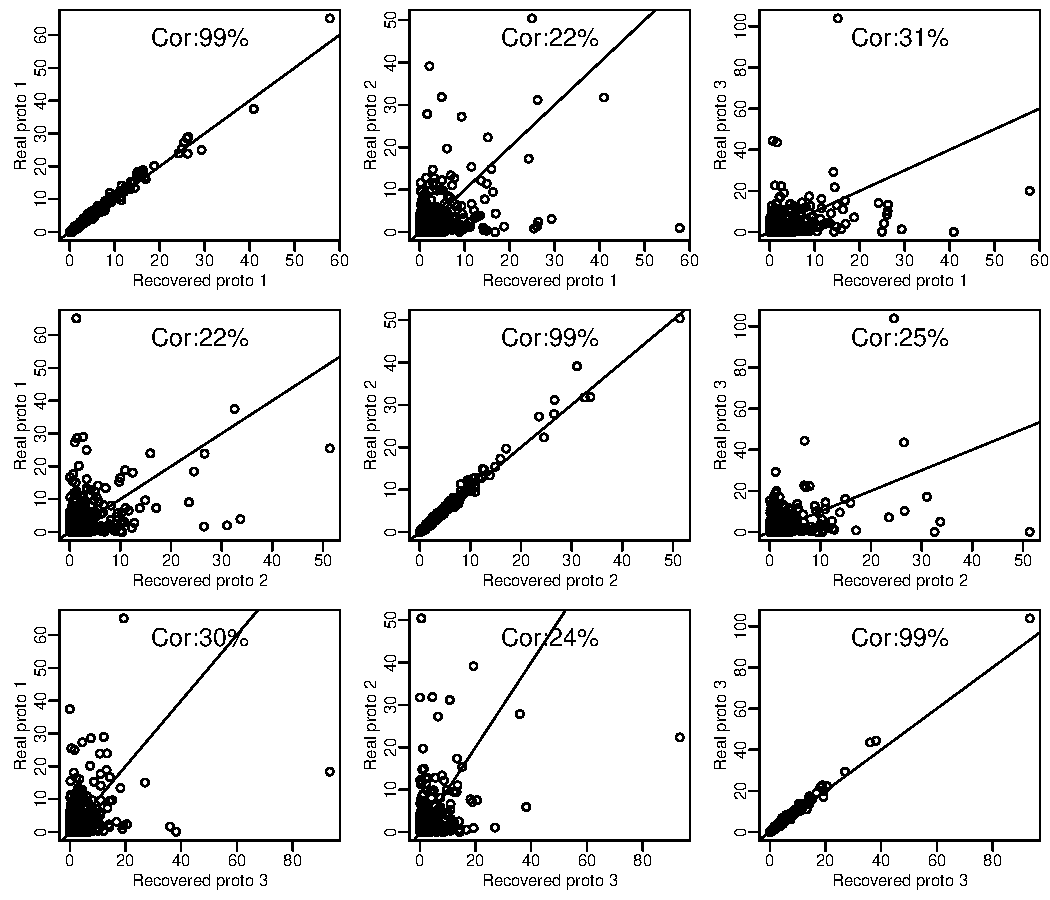
\includegraphics[width=\maxwidth]{figure/plotCorDeconv-1} 
\end{knitrout}

We do not typically know the number of factors in the mixture. The number of clusters will typically be larger than this. To simulate this, we use a kmeans with 4 groups.

\begin{knitrout}
\definecolor{shadecolor}{rgb}{0.969, 0.969, 0.969}\color{fgcolor}\begin{kframe}
\begin{alltt}
\hlstd{km} \hlkwb{=} \hlkwd{kmeans}\hlstd{(y,} \hlnum{4}\hlstd{,} \hlkwc{nstart}\hlstd{=}\hlnum{100}\hlstd{);}
\end{alltt}
\end{kframe}
\end{knitrout}

From this, we can use \verb!deconvoluteClusters! function to get the best mixture.
In this case the \verb!rmCutOff! parameter was increased to ensure that the bad cluster is removed, but that's not recommended in practice.
\begin{knitrout}
\definecolor{shadecolor}{rgb}{0.969, 0.969, 0.969}\color{fgcolor}\begin{kframe}
\begin{alltt}
\hlstd{dec2} \hlkwb{=} \hlkwd{deconvoluteClusters}\hlstd{(X, km}\hlopt{$}\hlstd{cluster,} \hlkwc{rmCutOff}\hlstd{=}\hlnum{.6}\hlstd{,} \hlkwc{mccores}\hlstd{=}\hlnum{7}\hlstd{,} \hlkwc{clean}\hlstd{=}\hlnum{FALSE}\hlstd{)}
\end{alltt}


{\ttfamily\noindent\itshape\color{messagecolor}{\#\# \ \ Kill:}}

{\ttfamily\noindent\itshape\color{messagecolor}{\#\# \ \ \ \ \ Iter:1}}

{\ttfamily\noindent\itshape\color{messagecolor}{\#\# \ \ \ \ \ Iter:2}}

{\ttfamily\noindent\itshape\color{messagecolor}{\#\# \ \ \ \ \ Iter:3}}

{\ttfamily\noindent\itshape\color{messagecolor}{\#\# \ \ \ \ \ Iter:4}}

{\ttfamily\noindent\itshape\color{messagecolor}{\#\# \ \ \ \ \ Iter:5}}

{\ttfamily\noindent\itshape\color{messagecolor}{\#\# \ \ \ \ \ Iter:6}}

{\ttfamily\noindent\itshape\color{messagecolor}{\#\# \ \ \ \ \ Iter:7}}

{\ttfamily\noindent\itshape\color{messagecolor}{\#\# \ \ \ \ \ Iter:8}}

{\ttfamily\noindent\itshape\color{messagecolor}{\#\# \ \ \ \ \ Iter:9}}

{\ttfamily\noindent\itshape\color{messagecolor}{\#\# \ \ \ \ \ Iter:10}}

{\ttfamily\noindent\itshape\color{messagecolor}{\#\# \ \ Full prototypes}}\end{kframe}
\end{knitrout}

The \verb!Kill! shown is list of cluters that are removed.
Note the calculation is done on a subset of 500 genes that fit the clustering well, then the prototypes  are calculated using \verb!NNMFproto! on all genes.

The clusters recovered can be extracted, their name corresponding to the indices of the original kmeans. The prototypes are a list with two items, \verb!proto! indicating the protoype values and \verb!sigma! giving the extra variance from the negative binomial.

\begin{knitrout}
\definecolor{shadecolor}{rgb}{0.969, 0.969, 0.969}\color{fgcolor}\begin{kframe}
\begin{alltt}
\hlstd{pr3} \hlkwb{=} \hlstd{dec2}\hlopt{$}\hlstd{proto}\hlopt{$}\hlstd{proto}
\hlkwd{show}\hlstd{(}\hlkwd{colnames}\hlstd{(pr3))}
\end{alltt}
\begin{verbatim}
## [1] "1" "2" "3" "4"
\end{verbatim}
\begin{alltt}
\hlkwd{show}\hlstd{(}\hlkwd{dim}\hlstd{(pr3))}
\end{alltt}
\begin{verbatim}
## [1] 500   4
\end{verbatim}
\end{kframe}
\end{knitrout}

We can check that the prototypes still fit well. Of course the ordering is random.

\begin{knitrout}
\definecolor{shadecolor}{rgb}{0.969, 0.969, 0.969}\color{fgcolor}\begin{kframe}
\begin{alltt}
\hlkwd{par}\hlstd{(}\hlkwc{mfrow}\hlstd{=}\hlkwd{c}\hlstd{(}\hlnum{3}\hlstd{,}\hlnum{3}\hlstd{),} \hlkwc{mar}\hlstd{=}\hlkwd{c}\hlstd{(}\hlnum{3}\hlstd{,}\hlnum{3}\hlstd{,}\hlnum{.5}\hlstd{,}\hlnum{.5}\hlstd{),} \hlkwc{mgp}\hlstd{=}\hlkwd{c}\hlstd{(}\hlnum{1.5}\hlstd{,}\hlnum{.5}\hlstd{,}\hlnum{0}\hlstd{))}
\hlkwa{for} \hlstd{(i} \hlkwa{in} \hlnum{1}\hlopt{:}\hlnum{3}\hlstd{)}
\hlstd{\{} \hlkwa{for} \hlstd{(j} \hlkwa{in} \hlnum{1}\hlopt{:}\hlnum{3}\hlstd{)}
  \hlstd{\{} \hlkwd{plot}\hlstd{(prot[,i], pr3[,j],} \hlkwc{xlab}\hlstd{=}\hlkwd{paste}\hlstd{(}\hlstr{"Recovered proto"}\hlstd{, i),}
      \hlkwc{ylab}\hlstd{=}\hlkwd{paste}\hlstd{(}\hlstr{"Real proto"}\hlstd{, j));} \hlkwd{abline}\hlstd{(}\hlnum{0}\hlstd{,}\hlnum{1}\hlstd{)}
    \hlkwd{mtext}\hlstd{(}\hlkwd{paste0}\hlstd{(}\hlstr{"Cor:"}\hlstd{,} \hlkwd{round}\hlstd{(}\hlkwd{cor}\hlstd{(prot[,i], pr3[,j],} \hlkwc{method}\hlstd{=}\hlstr{'s'}\hlstd{)}\hlopt{*}\hlnum{100}\hlstd{),} \hlstr{"%"}\hlstd{),} \hlkwc{side}\hlstd{=}\hlnum{3}\hlstd{,} \hlkwc{line}\hlstd{=}\hlopt{-}\hlnum{2}\hlstd{)}
  \hlstd{\}}
\hlstd{\}}
\end{alltt}
\end{kframe}
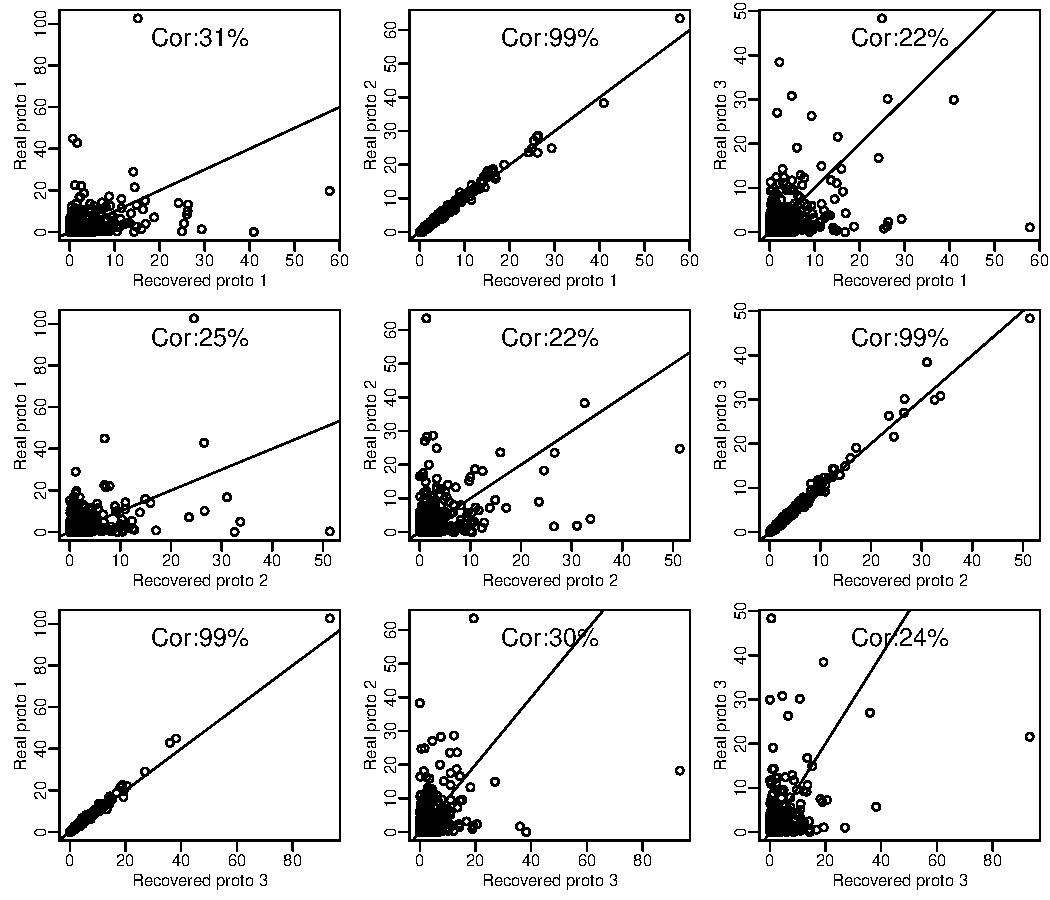
\includegraphics[width=\maxwidth]{figure/plotCorDeconv2-1} 
\end{knitrout}

\section{Recovery from another dataset}
%%%%%%%%%%%%%%%%%%%%%%
This is done via the \verb!getClustFrom! function.

\section{NNMF in other dataset}

This is quite similar, except it uses NNMF instead of negative binomial models.
This is done by using the \verb!NNMFother! function.

\subsection{Direct example}

As an example, imagine we have some sort of prototypes (4 prototypes, 100 genes) and mixing matrix (50 samples):

\begin{knitrout}
\definecolor{shadecolor}{rgb}{0.969, 0.969, 0.969}\color{fgcolor}\begin{kframe}
\begin{alltt}
\hlstd{prot} \hlkwb{=} \hlkwd{matrix}\hlstd{(}\hlkwd{rgamma}\hlstd{(}\hlnum{4}\hlopt{*}\hlnum{100}\hlstd{,} \hlnum{3}\hlstd{,} \hlnum{.01}\hlstd{),} \hlkwc{ncol}\hlstd{=}\hlnum{4}\hlstd{);} \hlkwd{rownames}\hlstd{(prot)} \hlkwb{=} \hlnum{1}\hlopt{:}\hlnum{100}\hlstd{;}
\hlstd{mix} \hlkwb{=} \hlkwd{matrix}\hlstd{(}\hlkwd{runif}\hlstd{(}\hlnum{4}\hlopt{*}\hlnum{50}\hlstd{)}\hlopt{^}\hlnum{2}\hlstd{,} \hlkwc{ncol}\hlstd{=}\hlnum{4}\hlstd{); mix} \hlkwb{=} \hlstd{mix}\hlopt{/}\hlkwd{rowSums}\hlstd{(mix)}
\end{alltt}
\end{kframe}
\end{knitrout}

The expected values are then just the product of the two

\begin{knitrout}
\definecolor{shadecolor}{rgb}{0.969, 0.969, 0.969}\color{fgcolor}\begin{kframe}
\begin{alltt}
\hlstd{e} \hlkwb{=} \hlstd{prot} \hlopt \hlkwd{t}\hlstd{(mix)}
\end{alltt}
\end{kframe}
\end{knitrout}

The observed values would then be taken from a Poisson distribution with those means

\begin{knitrout}
\definecolor{shadecolor}{rgb}{0.969, 0.969, 0.969}\color{fgcolor}\begin{kframe}
\begin{alltt}
\hlstd{obs} \hlkwb{=} \hlkwd{matrix}\hlstd{(}\hlkwd{rpois}\hlstd{(}\hlkwd{length}\hlstd{(e), e),} \hlkwc{ncol}\hlstd{=}\hlkwd{ncol}\hlstd{(e))}
\end{alltt}
\end{kframe}
\end{knitrout}

From \verb!obs! and \verb!prot!, we can easily recover the original mixture (correlations
are very close to 1):

\begin{knitrout}
\definecolor{shadecolor}{rgb}{0.969, 0.969, 0.969}\color{fgcolor}\begin{kframe}
\begin{alltt}
\hlstd{W} \hlkwb{=} \hlkwd{t}\hlstd{(}\hlkwd{nnlm}\hlstd{(prot, obs,} \hlkwc{loss}\hlstd{=}\hlstr{'mkl'}\hlstd{)}\hlopt{$}\hlstd{coefficients);}
\hlkwd{show}\hlstd{(}\hlkwd{diag}\hlstd{(}\hlkwd{cor}\hlstd{(W, mix)))}
\end{alltt}
\begin{verbatim}
## [1] 0.9987497 0.9986669 0.9991443 0.9989789
\end{verbatim}
\end{kframe}
\end{knitrout}

\subsection{In another study}

Now, the tricky part is that the genes in the new study are not on the same scale.
To simulate that, we add a scaling factor (here more or less between .1 and 10)

\begin{knitrout}
\definecolor{shadecolor}{rgb}{0.969, 0.969, 0.969}\color{fgcolor}\begin{kframe}
\begin{alltt}
\hlstd{scale} \hlkwb{=} \hlkwd{exp}\hlstd{(}\hlkwd{rnorm}\hlstd{(}\hlnum{100}\hlstd{));}
\end{alltt}
\end{kframe}
\end{knitrout}

This will give use new expected and observed values, as well as new recovered mixing coefficients (worse than previously):

\begin{knitrout}
\definecolor{shadecolor}{rgb}{0.969, 0.969, 0.969}\color{fgcolor}\begin{kframe}
\begin{alltt}
\hlstd{e2} \hlkwb{=} \hlstd{e} \hlopt{*} \hlstd{scale}
\hlstd{obs2} \hlkwb{=} \hlkwd{matrix}\hlstd{(}\hlkwd{rpois}\hlstd{(}\hlkwd{length}\hlstd{(e2), e2),} \hlkwc{ncol}\hlstd{=}\hlkwd{ncol}\hlstd{(e2));} \hlkwd{rownames}\hlstd{(obs2)} \hlkwb{=} \hlkwd{rownames}\hlstd{(e);}
\hlstd{W} \hlkwb{=} \hlkwd{t}\hlstd{(}\hlkwd{nnlm}\hlstd{(prot, obs2,} \hlkwc{loss}\hlstd{=}\hlstr{'mkl'}\hlstd{)}\hlopt{$}\hlstd{coefficients);}
\hlkwd{show}\hlstd{(}\hlkwd{diag}\hlstd{(}\hlkwd{cor}\hlstd{(W, mix)))}
\end{alltt}
\begin{verbatim}
## [1] 0.9400875 0.7480119 0.9664416 0.9904923
\end{verbatim}
\end{kframe}
\end{knitrout}

So this is where the \verb!NNMFother! function kicks in.

\begin{knitrout}
\definecolor{shadecolor}{rgb}{0.969, 0.969, 0.969}\color{fgcolor}\begin{kframe}
\begin{alltt}
\hlstd{fit} \hlkwb{=} \hlkwd{NNMFother}\hlstd{(obs2, prot)}
\hlkwd{show}\hlstd{(}\hlkwd{diag}\hlstd{(}\hlkwd{cor}\hlstd{(fit}\hlopt{$}\hlstd{W, mix)))}
\end{alltt}
\begin{verbatim}
## [1] 0.9989843 0.9988874 0.9990185 0.9992698
\end{verbatim}
\begin{alltt}
\hlkwd{show}\hlstd{(}\hlkwd{cor}\hlstd{(fit}\hlopt{$}\hlstd{sc, scale,} \hlkwc{method}\hlstd{=}\hlstr{'s'}\hlstd{))}
\end{alltt}
\begin{verbatim}
## [1] 0.9989559
\end{verbatim}
\end{kframe}
\end{knitrout}

And what if some genes (1 to 20) were just garbage?

\begin{knitrout}
\definecolor{shadecolor}{rgb}{0.969, 0.969, 0.969}\color{fgcolor}\begin{kframe}
\begin{alltt}
\hlstd{obs3} \hlkwb{=} \hlstd{obs2;}
\hlkwa{for} \hlstd{(i} \hlkwa{in} \hlnum{1}\hlopt{:}\hlnum{20}\hlstd{) \{ obs3[i,]} \hlkwb{=} \hlkwd{sample}\hlstd{(obs3[i,],} \hlkwc{replace}\hlstd{=}\hlnum{TRUE}\hlstd{) \}}
\hlstd{fit} \hlkwb{=} \hlkwd{NNMFother}\hlstd{(obs3, prot,} \hlkwc{maxIter}\hlstd{=}\hlnum{20}\hlstd{)}
\hlkwd{show}\hlstd{(}\hlkwd{diag}\hlstd{(}\hlkwd{cor}\hlstd{(fit}\hlopt{$}\hlstd{W, mix)))}
\end{alltt}
\begin{verbatim}
## [1] 0.9894250 0.9868811 0.9618847 0.9834111
\end{verbatim}
\begin{alltt}
\hlkwd{show}\hlstd{(}\hlkwd{cor}\hlstd{(fit}\hlopt{$}\hlstd{sc, scale,} \hlkwc{method}\hlstd{=}\hlstr{'s'}\hlstd{))}
\end{alltt}
\begin{verbatim}
## [1] 0.9987279
\end{verbatim}
\end{kframe}
\end{knitrout}

Results are substantially worse. It is however possible to judge how well each gene fits the NMF.

\begin{knitrout}
\definecolor{shadecolor}{rgb}{0.969, 0.969, 0.969}\color{fgcolor}\begin{kframe}
\begin{alltt}
\hlstd{r} \hlkwb{=} \hlstd{(prot}\hlopt{*}\hlstd{fit}\hlopt{$}\hlstd{sc)} \hlopt \hlkwd{t}\hlstd{(fit}\hlopt{$}\hlstd{W)}
\hlstd{cc} \hlkwb{=} \hlkwd{sapply}\hlstd{(}\hlnum{1}\hlopt{:}\hlkwd{nrow}\hlstd{(r),} \hlkwa{function}\hlstd{(}\hlkwc{i}\hlstd{)} \hlkwd{cor}\hlstd{(r[i,], obs3[i,],} \hlkwc{method}\hlstd{=}\hlstr{'s'}\hlstd{))}
\hlkwd{show}\hlstd{(}\hlkwd{fivenum}\hlstd{(cc[}\hlnum{1}\hlopt{:}\hlnum{20}\hlstd{]))}
\end{alltt}
\begin{verbatim}
## [1] -0.17499576 -0.02385935  0.07495179  0.13437735  0.33434267
\end{verbatim}
\begin{alltt}
\hlkwd{show}\hlstd{(}\hlkwd{fivenum}\hlstd{(cc[}\hlnum{21}\hlopt{:}\hlnum{100}\hlstd{]))}
\end{alltt}
\begin{verbatim}
## [1] 0.1067448 0.8006673 0.9046835 0.9463207 0.9879229
\end{verbatim}
\end{kframe}
\end{knitrout}

The correlation of OK genes is much higher. If we redo the analysis on only the genes with correlation of at least \verb!0.7!

\begin{knitrout}
\definecolor{shadecolor}{rgb}{0.969, 0.969, 0.969}\color{fgcolor}\begin{kframe}
\begin{alltt}
\hlstd{w} \hlkwb{=} \hlstd{cc}\hlopt{>}\hlnum{.7}\hlstd{;}
\hlstd{fit} \hlkwb{=} \hlkwd{NNMFother}\hlstd{(obs3[w,], prot[w,],} \hlkwc{maxIter}\hlstd{=}\hlnum{20}\hlstd{)}
\hlkwd{show}\hlstd{(}\hlkwd{diag}\hlstd{(}\hlkwd{cor}\hlstd{(fit}\hlopt{$}\hlstd{W, mix)))}
\end{alltt}
\begin{verbatim}
## [1] 0.9989343 0.9985187 0.9988844 0.9992216
\end{verbatim}
\end{kframe}
\end{knitrout}

Of course here the 0.7 cutoff is arbitrary and somewhat optimized.


\section{Conclusion}
%%%%%%%%%%%%%%%%%%%%%%


\end{document}
